\begin{frame}[t]
\frametitle{Some traffic statistics \dots}
    Are we improving the conditions?
    \hspace{-0.1cm}
    \begin{center}
    \begin{columns}[t]
      \begin{column}{0.5\textwidth}
      \begin{figure}
      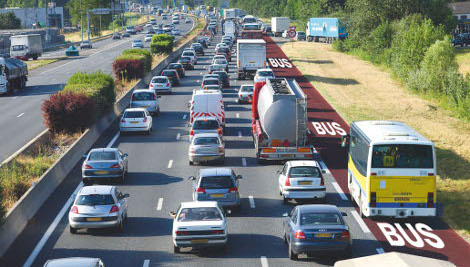
\includegraphics[width = 0.9\textwidth]{fig_37_grenoble-traffic}
      \end{figure}
      \metroset{block=fill}
      \uncover<2->{
      \begin{alertblock}{Now $\rightarrow$}
        \begin{itemize}
          \item[\frownie] {\small Cities tend to get more urban.}
          \item[\smiley] {\small Big sources of data.}
          \item[\smiley] {\small New measurements available for this purpose (e.g. GPS).}
        \end{itemize}
      \end{alertblock}
      }
    \end{column}
    \begin{column}{0.5\textwidth}
    \uncover<3>{
      \begin{exampleblock}{Inrix}
      Lyon: In 2014 drivers waste 36.03 (40H \~ 2013) hours per year in traffic,
      Worst Hour = Tuesday 08:00-09:00 \footnote[frame]{\href{http://inrix.com/press-releases/2661/}{INRIX Report 2014}}
      \end{exampleblock}
      \begin{alertblock}{Current condition!}
      France has moved from 4th to 7th position in the list of most congested countries in Europe with 29 lost hours in congestion during congestions in 2014 -  6th in the last report in 2016\footnote[frame]{\href{http://inrix.com/press-releases/scorecard-report-france/}{INRIX Report 2015}}.
      \end{alertblock}
    }
      \end{column}
    \end{columns}
    \end{center}
\end{frame}